\documentclass[10.5pt,a4paper]{article}
\usepackage{xltxtra}
%--tikz related>
\usepackage{tikz}
\usetikzlibrary{shadows,shapes,arrows,arrows.meta,chains}
\usetikzlibrary{calc}
\usetikzlibrary{math}
\usetikzlibrary{intersections} % provide name path and name intersections option for \path
%<---
%->->->->->->->->->->->->->->->->->->->->->->
\usepackage{varwidth} % 在刘海洋的书中,5.3.3章节,varwidth用于让两个图片顶部对齐,详细看书5.3.3
%<-<-<-<-<-<-<-<-<-<-<-<-<-<-<-<-<-<-<-<-<-<-
%->->->->->->->->->->->->->->->->->->->->->->->->->->->->->->
% hyperref 会生成书签和目录超链接
% citecolor设置引用时数字的颜色
\usepackage[colorlinks,linkcolor=black,citecolor=black]{hyperref}
\hypersetup{
bookmarksnumbered
}
\usepackage{nameref}
%<-<-<-<-<-<-<-<-<-<-<-<-<-<-<-<-<-<-<-<-<-<-<-<-<-<-<-<-<-<-

%->->->->->->->->->->->->->->->->->->->->->->->->->->->->->->三线表格
\usepackage{booktabs}
%<-<-<-<-<-<-<-<-<-<-<-<-<-<-<-<-<-<-<-<-<-<-
%->->->->->->->->->->->->->->->->->->->->->->
\usepackage{tocloft}
\renewcommand\cftsecleader{\cftsubsecleader}
%<-<-<-<-<-<-<-<-<-<-<-<-<-<-<-<-<-<-<-<-<-<-<-<-<-<-<-<-<-<-

%->->->->->->->->->->->->->->->->->->->->->->
\usepackage{comment}
%<-<-<-<-<-<-<-<-<-<-<-<-<-<-<-<-<-<-<-<-<-<-<-<-<-<-<-<-<-<-

%->->->->->->->->->->->->->->->->->->->->->->
\usepackage[numbers,square]{natbib}
\setcitestyle{super} %如果想在正文中的引用为上标形式,用super。引用的方括号和正文一样大小,注释此行。
%\bibliographystyle{plainnat}
    %\bibliographystyle{unsrtnat}
\bibliographystyle{cumtunsrtnat}
\renewcommand*{\bibfont}{\fontsize{10.5pt}{12pt}\selectfont }
%<-<-<-<-<-<-<-<-<-<-<-<-<-<-<-<-<-<-<-<-<-<-
\usepackage{float}
\usepackage{wrapfig} % used for \begin{wrapfigure} and \begin{wraptable}, 刘海洋的书5.3.5有介绍
%->->->->->->->->->->->->->->->->->->->->->->
\usepackage{amsmath}
% 每个section的图和表重新编号
\numberwithin{equation}{section}
\numberwithin{figure}{section}
\numberwithin{table}{section}
\renewcommand\theequation{\arabic{section}-\arabic{equation}}
\renewcommand\thefigure{\arabic{section}-\arabic{figure}}
\renewcommand\thetable{\arabic{section}-\arabic{table}}
\usepackage{amssymb} %输出比如数学空集、交集等各种符号
\usepackage[all,pdf]{xy} % provide\xymatrix{}
\usepackage{pstricks}
\usepackage{pstricks-add} % 相当于:\usepackage{pst-plot,pst-node}
%<-<-<-<-<-<-<-<-<-<-<-<-<-<-<-<-<-<-<-<-<-<-
%->->->->->->->->->->->->->->->->->->->->->->
\usepackage{caption,subcaption} % for captionsetup, subcaption用于插入多个图片时,有一个总标题,各个小图片有各自的小标题
%<-<-<-<-<-<-<-<-<-<-<-<-<-<-<-<-<-<-<-<-<-<-
\DeclareCaptionLabelSeparator{space}{\ \ \ \ }
\captionsetup{labelsep=space} % 效果是图片、表格的标题变成: 图2: this is. 2与this之间是空格
%\captionsetup{labelsep=space, figurewithin=section} % 效果是图片、表格的标题变成: 图2: this is. 2与this之间是空格

\usepackage{ctex}
\usepackage{graphicx}
\usepackage{titlesec}
\setlength{\unitlength}{1mm}


\usepackage{indentfirst}
\setlength{\parindent}{2em}
%->->->->->->->->->->->->->->->->->->->->->->
% 设置上下左右页边距,设置页眉与页边距离:上页边-页眉边距=headsep, 刘海洋书page 145
% LaTeX左边页边距=word左页边距+word装订线距离
\usepackage{geometry}
%\geometry{left=2cm,right=2cm,top=2cm,bottom=2cm,headsep=0.5cm}
%\geometry{left=2.5cm,right=2cm,top=2.3cm,bottom=2cm,headsep=0.2cm}
% 教务部:
%\geometry{left=2.5cm,right=2cm,top=2.4cm,bottom=2cm,headsep=0.2cm,footskip=0.5cm}
\geometry{left=2.5cm,right=2cm,top=2.4cm,bottom=2.5cm,headsep=0.2cm,footskip=0.7cm}
%<-<-<-<-<-<-<-<-<-<-<-<-<-<-<-<-<-<-<-<-<-<-

%->->->->->->->->->->->->->->->->->->->->->->
\setmainfont{Times New Roman}
\setCJKmainfont{SimSun}

\setCJKfamilyfont{song}{SimSun}
\setCJKfamilyfont{hei}{SimHei}
\setCJKfamilyfont{kai}{KaiTi}
\newcommand{\song}{\CJKfamily{song}}
\newcommand{\hei}{\CJKfamily{hei}}
\newcommand{\kai}{\CJKfamily{kai}}
%<-<-<-<-<-<-<-<-<-<-<-<-<-<-<-<-<-<-<-<-<-<-



%->->->->->->->->->->->->->->->->->->->->->->
\usepackage{fancyhdr}
%\pagestyle{fancy}
%\pagenumbering{arabic}
%\fancyhf{}
%\renewcommand{\headrulewidth}{1pt}
\pagestyle{fancy}
\pagenumbering{Roman}
\fancyhf{}
\fancyfoot[C]{\fontsize{9pt}{\baselineskip}\selectfont\thepage}
\renewcommand{\headrulewidth}{0pt}

%<-<-<-<-<-<-<-<-<-<-<-<-<-<-<-<-<-<-<-<-<-<-

%->->->->->->->->->->->->->->->->->->->->->->
%中文相关
\renewcommand{\figurename}{图}
%\renewcommand{\refname}{\centerline{文章参考文献}}
\renewcommand\refname{{\hei\bfseries\fontsize{18pt}{\baselineskip}\selectfont\centerline{参考文献}}} % 四号,黑体,顶格
\renewcommand\contentsname{{\hei\bfseries\fontsize{18pt}{\baselineskip}\selectfont\centerline{目\qquad 录}}}%让目录标题居中,1. \centerline{目录}2.\hspace{\fill},可以实现左、中、右对齐,更灵活
%\renewcommand{\contentsname}{\hspace{\fill}本文的目录\hspace{\fill}}
%<-<-<-<-<-<-<-<-<-<-<-<-<-<-<-<-<-<-<-<-<-<-

%->->->->->->->->->->->->->->->->->->->->->->
% \titleformat{ <command > }[<shape >]{<format >}{<label >}{<sep >}{<before >}[<after >]
%\titleformat{\section} [hang] { \centering\hei \fontsize{15pt}{\baselineskip}\selectfont } {\thesection} {1em} {}
% 学校突然又不要居中了, fuck, 另外一级标题他要加粗,尝试发现,加粗太丑了,就没有加粗
\titleformat{\section} [hang] {\bfseries\hei\fontsize{18pt}{\baselineskip}\selectfont } {\thesection} {1em} {}
%\titleformat{\section} [hang] {\hei\fontsize{18pt}{\baselineskip}\selectfont } {\thesection} {1em} {}
\titleformat{\subsection} [hang] { \hei \fontsize{15pt}{\baselineskip}\selectfont } {\thesubsection} {1em} {}
\titleformat{\subsubsection} [hang] {\hei\fontsize{14pt}{\baselineskip}\selectfont } {\thesubsubsection} {1em} {}
% <before> is code preceding the title body. The very last command can take an argument, which is the title text.
%\titleformat{\subsection} [hang]      {\hei\large}{\raisebox{-1mm}[0pt]{\linethickness{0.3mm}\put(-1,0){\line(1,0){141}}\linethickness{1.5mm}\put(140,0){\line(1,0){1.5}}}\bf{\thesubsection}}{1em}{}
%\titleformat{\subsection} [hang]      {\hei\large}{\raisebox{-1mm}[0pt]{\linethickness{0.3mm}\linethickness{1.5mm}}\bf{\thesubsection}}{1em}{}
%<-<-<-<-<-<-<-<-<-<-<-<-<-<-<-<-<-<-<-<-<-<-
\begin{document}
% 双语目录http://blog.csdn.net/solstice/article/details/1589348
\makeatletter
\newcommand\engcontentsname{\sffamily\fontsize{18pt}{\baselineskip}\selectfont\centerline{\textbf{Contents}}}
\newcommand\tableofengcontents{%
    \if@twocolumn
      \@restonecoltrue\onecolumn
    \else
      \@restonecolfalse
    \fi
    \section*{\engcontentsname
        \@mkboth{%
           \MakeUppercase\engcontentsname}{\MakeUppercase\engcontentsname}}%
    \@starttoc{toe}% !!!!Define a new contents!!!!
    \if@restonecol\twocolumn\fi
    }
\newcommand\addengcontents[2]{%
    \addcontentsline{toe}{#1}{\protect\numberline{\csname the#1\endcsname}#2}}
\makeatother

\newcommand\echapter[1]{\addengcontents{chapter}{#1}}
\newcommand\esection[1]{\addengcontents{section}{#1}}
\newcommand\esubsection[1]{\addengcontents{subsection}{#1}}
% self
\newcommand\etitlesection[1]{{\noindent\bfseries\fontsize{18pt}{\baselineskip}\selectfont\noindent\thesection\hspace{1em}#1\par\vspace{1em}}}
\newcommand\etitlesubsection[1]{{\noindent\hei\fontsize{15pt}{\baselineskip}\selectfont\thesubsection\hspace{1em}#1\par\vspace{1em}}}
% end of 双语目录http://blog.csdn.net/solstice/article/details/1589348
\newcommand\mmx{\mathrm{x}}
\setcounter{tocdepth}{2}
\phantomsection
\addcontentsline{toc}{section}{摘要}
{\centering \hei \fontsize{18pt}{\baselineskip}\selectfont 摘\qquad 要\par}
\vspace{1em}
% 12pt字号大致是小四,行距18pt大致与word的20磅相同
\fontsize{12pt}{18pt}\selectfont
红外热成像技术作为一种可以全天工作的成像技术,在军事、工业和民用等领域都有着广泛的应用。由于设备的限制,红外图像的视角比较窄,分辨率比较低,%
基于红外图像的特征提取与图像拼接算法可以解决当前红外图像视角窄的问题。\par
%摘要修改的余地小
本文以SIFT特征为基础,研究了红外图像的特征提取、特征匹配和图像融合相关算法,最终通过图像拼接实验验证了图像拼接算法的可行性。\par
\vspace{2em}
\par
该论文有图xx幅,表xx个,参考文献xx篇。
\par
\noindent \textbf{关键词:}SIFT; 特征提取; 特征匹配; 图像融合; 图像拼接
\par
					\newpage %英文摘要
\phantomsection
\addcontentsline{toe}{section}{Abstract}
{\centering \hei \fontsize{18pt}{\baselineskip}\selectfont\bfseries \textsf{Abstract}\par}
%\fontsize{12pt}{\baselineskip}\selectfont %英文摘要及关键字 小四号
\fontsize{12pt}{16pt}\selectfont
As an imaging technology which can work all day, infrared thermal imaging technology has a wide range of applications in military, industrial and civilian areas.
Due to the limitation of the equipment, the infrared image has a narrow viewing angle and the resolution is relatively low. The feature extraction and image mosaic algorithm based on infrared image can solve the problem that the viewing angle of infrared image is narrow.
%equipment不可数名词
\par
Based on the SIFT feature, this paper studies the feature extraction, feature matching and image fusion algorithm of infrared image. Finally, the feasibility of image mosaic algorithm is verified by image mosaic experiment.%
\par
\vspace{2em}
\par
\noindent \textbf{Keywords:} SIFT; feature extraction; feature matching; image fusion; image mosaic
% 中文目录
\newpage
\phantomsection
\addcontentsline{toc}{section}{目录}
\tableofcontents
% end of中文目录
% 英文目录
\newpage
\phantomsection
\addcontentsline{toe}{section}{Contents}
\tableofengcontents
% end of 英文目录
\newpage % 开始正文
% -->
\pagestyle{fancy}
\pagenumbering{arabic}
\fancyhf{}
\fancyhead[C]{\fontsize{10.5pt}{\baselineskip}\selectfont \leftmark}
\fancyfoot[C]{\fontsize{9pt}{\baselineskip}\selectfont\thepage}
%\renewcommand{\headrulewidth}{1pt}
\renewcommand{\headrulewidth}{0.5pt}
% <--
\setcounter{page}{1}
% 学校的奇葩要求:行距18磅,完全是M$ word的标准
\fontsize{12pt}{16pt}\selectfont
\section{绪论\label{sectionXulun}}
\esection{Introduction}
\etitlesection{Introduction}
\subsection{本课题的研究目的和意义}
\esubsection{The purpose and significance of this research}
\etitlesubsection{The purpose and significance of this research}
自2017届毕业生开始,中国矿业大学本科生毕业论文的格式要求变得比以前更加规范了,本\LaTeX{}模板是由个人根据中国矿业大学本科毕业论文的要求%
逐渐调整最终达到和word在字体、字号、页边距、页眉页脚距离等要求基本一致的效果的一个模板。
学校给过一个本科论文的模板,毫无疑问,学校给的模板是word的。
而且,对格式的要求比如行距多少磅、字号大小等,都是采用的微软公司的word的标准,而\LaTeX{}在这些参数方面和word的标准是不一样。
\par
所以,调整格式的整个过程是比较繁琐的,希望本模板可以减少以后需要使用\LaTeX{}写毕业论文的矿大本科毕业生的工作量,专注于内容,减少在格式上消耗的时间。
本人在离开学校后把这个模板(姑且称为模板吧,本人\LaTeX{}水平并不高,跟THU、SJTU、USTC、XJTU等高校的牛人做出来的模板比起来,差的太远了,惭愧)分享出来,算是%
在离开之后留下一些东西吧。
\par
本模板的中文解决方案是\XeLaTeX{}+ctex宏包,源文件编码为UTF8,推荐安装texlive,基本所有的宏包都有了。
./simpleMake.sh是进行一次编译的, ./clean.sh是清除日志等各种辅助文件的。
./make.sh是进行完整编译的,并包含几条sed命令,这是因为生成的个别参考文献无法完全满足矿大本科毕业论文的要求。
而bibtex管理参考文献时采用bst文件定义格式,该文件采用逆波兰表示法,个人感觉是一种反人类的令人痛苦的语法,与其修改bst文件,不如用sed结合正则表达式直接改.bbl文件来的快。\par
关于参考文献的管理,使用bibtex管理参考文献,需要把本目录中的cumtunsrtnat.bst放在texlive的安装目录下,和texlive自己的unsrtnat.bst在同一个目录。
比如,我的是在\verb|D:\Bin\texlive\texlive2016\texmf-dist\bibtex\bst\natbib|下。\par
其实这个cumtunsrtnat.bst和texlive自己的unsrtnat.bst区别很小,我只是在unsrtnat.bst的基础上修改了少量的几行。
\par
如果不想使用本目录下的几个shell小脚本编译,直接一条一条敲命令也是可以的,当然使用IDE也行,这根据个人喜好。我自己是安装了windows版的git,该软件自
带一个终端模拟器git-bash,还提供了sed、grep、awk、find等强大的unix命令,连perl都有,非常好用。编辑器采用vim(也是windows版的git提供的),notepad++也比较好,根据自己喜好选择自己的编辑器吧。像毕业论文这样的大工程,还是有一个版本控制
工具比较好,随时查看历史版本,我用的是git,大家也可以用自己喜欢的。自从有了git,后悔药不再是梦想。
\par
在图像拼接过程中,确定图像间的位置关系是比较关键的一个步骤。图像拼接的效果在很大程度上受位置关系的精度的影响\cite{zagrouba2009efficient,chen2014optimization}。\par
\subsection{国内外研究状况}
\esubsection{Research status at home and abroad}
\etitlesubsection{Research status at home and abroad}
图像拼接的过程,不同的学者有不同的划分方法,但总体方向是不会有太大的差别的,关键环节主要包括特征提取、特征匹配和图像融合。
\newpage
\section{SIFT算法\label{sectionSift}}
\esection{SIFT algorithm}
\etitlesection{SIFT algorithm}

\subsection{尺度空间极值检测}
\esubsection{Scale-space exetrema detection}
\etitlesubsection{Scale-space exetrema detection}

简单的数学公式示例:\par
只有一种线性核可以用于实现尺度变换,它就是高斯核,这已经得到Linderberg等人的证明\cite{lindeberg1994scale}。
尺度空间$L(x,y,\sigma)$表示如下:
\begin{equation}
L(x,y,\sigma) = G(x,y,\sigma) * I(x,y)
\end{equation}
\par
其中,$I(x,y)$为待处理图像,$*$代表卷积运算,$G(x,y,\sigma)$为高斯函数\cite{lowe2004distinctive}。对于二维情形,高斯函数形式如下:
\begin{equation}
G(x,y,\sigma) = \frac{1}{2\pi\sigma^2}e^{-(x^2+y^2)/(2\sigma^2)}
\end{equation}
\subsubsection{高斯差分金字塔}
\par
高斯差分金字塔中的层是由高斯金字塔中相邻的层相减得到的,在得到高斯差分金字塔前,要先构造出高斯金字塔。
其组数$octv$由下式确定:
\begin{equation}
octv = \log_2\{min(M,N)\}-t, t\in[0,\log_2\{min(M,N)\})
\end{equation}
\par
再来个简单的插图与引用图的示例:\par
如图\,\ref{gaussianAndDog}\,所示,右边就是高斯差分金字塔,从图中可以看出它的形成过程。
\begin{figure}[htbp]
\centering
				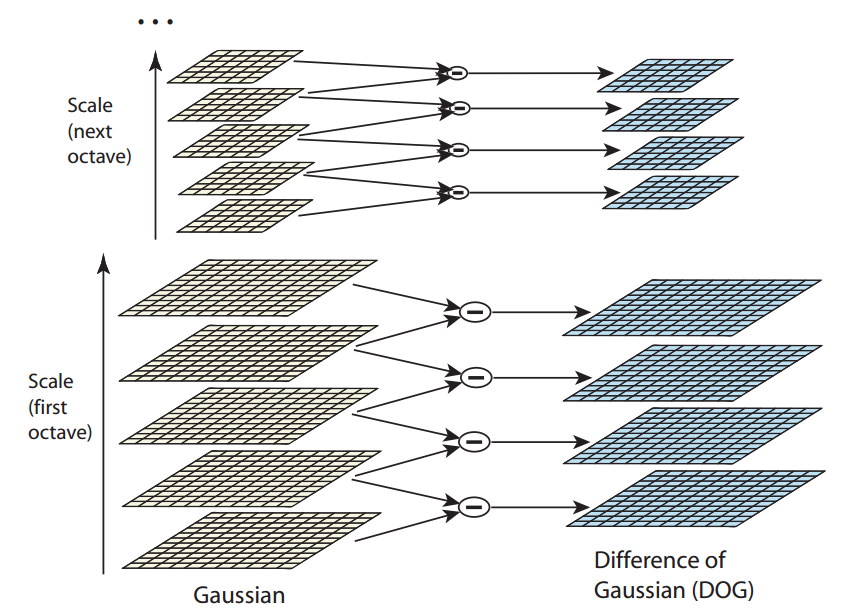
\includegraphics[width=.8\textwidth]{gaussianAndDog.PNG}
\caption{左边相邻层图像两两相减得到右边图像\cite{lowe2004distinctive}。\label{gaussianAndDog}}
\addtocounter{figure}{-1}
\renewcommand{\figurename}{Figure}
\caption{Adjacent images on the left is subtracted each other to get images on the right\cite{lowe2004distinctive}.}
\end{figure}
\subsection{关键点精确定位}
\esubsection{Keypoint localization}
\etitlesubsection{Keypoint localization}
\subsubsection{关键点的插值计算}
在插值计算这一步聚中,有一些点的像素值太小了,这些点应该被舍弃,因为像素值过小的点抗干扰能力比较弱\cite{lowe2004distinctive}。
对DoG函数进行展开,有:
\begin{equation}
\label{taylorD}
D(\mathrm{x}) = D + \frac{\partial{D}^T }{\partial \mathrm{x}} \mathrm{x} + \frac 12 \mathrm{x}^T \frac{\partial^2D}{\partial \mathrm{x}^2}\mathrm{x}
\end{equation}
简单的矩阵排版示例:\par
其中,$\mmx=[x,y,\sigma]^T$,而$\frac{\partial D }{\partial\mathrm{x} }$和$\frac{\partial^2 D}{\partial \mathrm{x}^2}$的计算方法如式(\ref{hessianMatrix})所示。
\begin{equation}
\label{hessianMatrix}
\frac{\partial D}{\partial\mmx} = 
\begin{bmatrix}
\frac{\partial D}{\partial x} \\
\frac{\partial D}{\partial y}  \\
\frac{\partial D}{\partial \sigma}  \\
\end{bmatrix}
,\,
\frac{\partial^2 D}{\partial \mathrm{x}^2} = \begin{bmatrix}
\frac{\partial^2 D}{\partial x^2} &\frac{\partial^2 D}{\partial x\partial y}  &\frac{\partial^2 D}{\partial x\partial\sigma} \\
\frac{\partial^2 D}{\partial y\partial x} &\frac{\partial^2 D}{\partial y^2}  &\frac{\partial^2 D}{\partial y\partial\sigma} \\
\frac{\partial^2 D}{\partial\sigma\partial x} &\frac{\partial^2 D}{\partial\sigma\partial y}  &\frac{\partial^2 D}{\partial\sigma^2} \\
\end{bmatrix}
\end{equation}
\par
\begin{equation}
\mathbf{H} = \begin{bmatrix}
D_{xx}  & D_{xy}\\
D_{xy} & D_{yy}\\
\end{bmatrix}
\end{equation}
\par
多行公式一个编号:\par
\begin{align}
D_{xx}= &D(x+1,y)+D(x-1,y)-2D(x,y) \notag\\
D_{xy}= &\frac{D(x-1,y-1)+D(x+1,y+1)-D(x+1,y-1)-D(x-1,y+1)}{4}\\
D_{yy}= & D(x,y+1)+ D(x,y-1) -2D(x,y) \notag
\end{align}
\par
如果插图中有多个子图,目前我所知道的灵活性最大的方法是使用subfigure环境。
可给图加标题和子标题,子标题的位置可上可下,引用图的编号时可分别引用图和子图,具体操作请看源代码。
\par
下面的实验说明了上面这些处理的效果。如图\,\ref{compareThresholdAndEdgeResponse}\,所示。
图\ref{compareThresholdAndEdgeResponse}(\subref{originalZhulou})是原始图像。
\begin{figure}[htbp]
\centering
	\begin{subfigure}[b]{.4\textwidth}
		\centering
				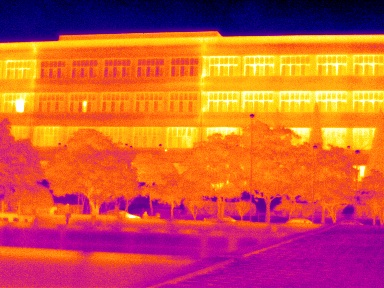
\includegraphics[width=\textwidth]{useful/compareEdgeResponse/12.jpg}
				\caption{原始图像\label{originalZhulou}}
				\addtocounter{subfigure}{-1}
				\caption{Original image}
	\end{subfigure}
	\qquad
	\begin{subfigure}[b]{.4\textwidth}
		\centering
				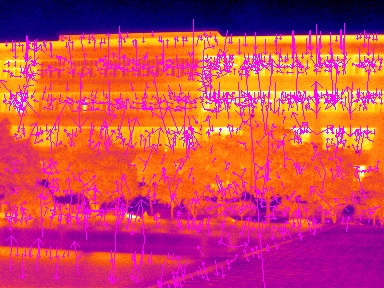
\includegraphics[width=\textwidth]{useful/compareEdgeResponse/siftFeature1301.jpg}
				\caption{初步检测极值点\label{noContrTh}}
				\addtocounter{subfigure}{-1}
				\caption{Initial detection of extrema}
	\end{subfigure}
%	\\
	\begin{subfigure}[b]{.4\textwidth}
		\centering
				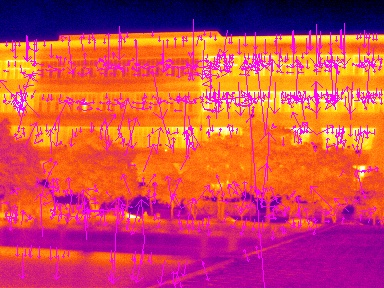
\includegraphics[width=\textwidth]{useful/compareEdgeResponse/siftFeature918.jpg}
				\caption{灰度值过低的点被去除以后\label{noEdgeElimit}}
				\addtocounter{subfigure}{-1}
				\caption{Points whose gray scale value is too low are removed}
	\end{subfigure}
	\qquad
	\begin{subfigure}[b]{.4\textwidth}
		\centering
				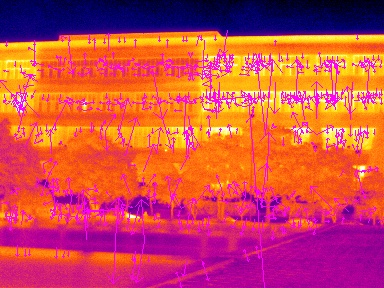
\includegraphics[width=\textwidth]{useful/compareEdgeResponse/siftFeature792.jpg}
				\caption{消除边缘响应以后\label{withEdgeElimit}}
				\addtocounter{subfigure}{-1}
				\caption{After the edge response is eliminated\vspace{1.5em}}
	\end{subfigure}
\caption{逐渐剔除不稳定点的过程。其中,(\subref{noContrTh})中有1301个关键点,(\subref{noEdgeElimit})中有918个关键点,(\subref{withEdgeElimit})中有792个关键点。\label{compareThresholdAndEdgeResponse}}
\addtocounter{figure}{-1}
\renewcommand{\figurename}{Figure}
\caption{The process of eliminating unstable points. There is 1301 keypoints is (\subref{noContrTh}), 918 keypoints in
(\subref{noEdgeElimit}), 792 keypoints in (\subref{withEdgeElimit}).}
\end{figure}
\par
tikz宏包是一个非常强大的画图宏包,文档就有1100多页,这里给出一个简单的例子。\par
将坐标轴旋转一定角度以使$x$轴的方向与特征点的幅值最大的方向保持一致。这样,提取出的特征点不会随着图像的角度的变化而变化,图\,\ref{rotateAxesjpg}\,给出了旋转前后的对比。
\begin{figure}[htbp]
\centering
% use layer
% --->
\pgfdeclarelayer{background}
\pgfdeclarelayer{foreground}
\pgfsetlayers{background,main,foreground}
\begin{tikzpicture}[>=Stealth,scale=0.8]
% left
\draw(-3.536,-3.536)rectangle(3.536,3.536);
\draw(0,0)circle(3.536);
\draw[->,thick](-3.536,0)--(3.536,0);
\draw[<-,thick](0,-3.536)--(0,3.536);
\node[above]at(3.3,0){$x$};
\node[right]at(0,-3.3){$y$};
\begin{scope}[xshift=-2.5cm,yshift=-2.5cm]
\draw[dashed,step=1] (0,0) grid (5,5);
\end{scope}
\begin{pgfonlayer}{foreground}
\draw[very thick,->,rotate=-30](0,0)--(2,0);
\end{pgfonlayer}
\begin{pgfonlayer}{background}
%\fill[rotate=-30,gray!10](0,0)--(-1,-1)--(2,0)--(-1,1)--cycle;
\fill[rotate=-30,gray!20](0,0)--(-1,-1)--(2,0)--(-1,1)--cycle;
\end{pgfonlayer}
%\draw[->,very thick](4.5,0)--(6.5,0);
\filldraw(4.5,-0.1cm)rectangle(6.3,0.1cm);
\filldraw(6.3,-0.3)--(6.6,0)--(6.3,0.3);
% right
\begin{scope}[xshift=11cm]
\draw(-3.536,-3.536)rectangle(3.536,3.536);
\draw(0,0)circle(3.536);
	\begin{scope}[rotate=-30]
	\node[rotate=-30,above]at(3.3,0){$x$};
	\node[rotate=-30,right]at(0,-3.3){$y$};
	\draw[->,thick](-3.536,0)--(3.536,0);
	\draw[<-,thick](0,-3.536)--(0,3.536);
		\begin{scope}[xshift=-2.5cm,yshift=-2.5cm]
		\draw[dashed,step=1] (0,0) grid (5,5);
		\end{scope}
	\end{scope}
\begin{pgfonlayer}{foreground}
\draw[->,rotate=-30,very thick](0,0)--(2,0);
\end{pgfonlayer}
%
\begin{pgfonlayer}{background}
\fill[rotate=-30,gray!20](0,0)--(-1,-1)--(2,0)--(-1,1)--cycle;
\end{pgfonlayer}
\end{scope}
\end{tikzpicture}
% <---
\caption{旋转坐标轴。\label{rotateAxesjpg}}
\addtocounter{figure}{-1}
\renewcommand{\figurename}{Figure}
\caption{Rotate the axis.}
\end{figure}
\newpage
\section{特征匹配\label{sectionKdMatch}}
\esection{Feature matching}
\etitlesection{Feature matching}
这里给出一个用tikz宏包画流程图的例子:\par
构造$k\text{-}d$树的流程如图~\ref{liucheng_buildkdtree}~所示。
\begin{figure}[htbp]
\centering
% --> tree
\tikzstyle{line}     = [draw, thick, color=black, -latex']
\tikzstyle{proc} = [rectangle,draw,text width=6em, text centered,minimum height=3em]
\tikzstyle{term} = [proc,rounded corners]
\tikzstyle{test} = [proc,diamond,inner sep=-3pt]
\begin{tikzpicture}[scale=0.7,transform shape]
  \path node(p1)[term]{特征点数据\\ features};
  \path (p1.south)+(0,-1) node(p2)[proc]{展开$k\text{-}d$树};
\path (p2.south)+(0,-1) node(p3)[proc,text width=10em]{选择最大方差维数ki\\Assign Partition Key};
\path(p3.south)+(0,-1) node(p4)[proc,text width=12em](p4){选取ki维中值kv作阈值\\Median Select};
\path(p4.south)+(0,-2)         node(p5)[test,aspect=2,text width=10em]{分割数据\\Partition Feature};
    %  \path (p5.south)+(-3.5,-1.5) node(p61)[proc]{左特征点数据\\features};
    \path (p5.south)+(-3.5,-1.5) node(p61)[term]{左特征点数据\\features};
  \path (p5.south)+(3.5,-1.5) node(p62)[term]{右特征点数据\\features};
\path (p61.south)+(0,-1) node(p71)[proc]{展开左子树};
\path (p62.south)+(0,-1) node(p72)[proc]{展开右子树};
%\node[test,join,text width=10em](t1) {t1:分割数据\\Partition Feature?};
% line
  \path [line] (p1.south) -- (p2);
  \path [line] (p2.south) -- (p3);
  \path [line] (p3.south) -- (p4);
  \path [line] (p4.south) -- (p5);
%  \path [line] (p5.west) -- +(-0.5,0) -- (p61);
  \path [line] (p5.west)-| node[near start, yshift=-2em,fill=white]{$ki$维$\le kv$}(p61);
  \path [line] (p5.east)-| node[near start, yshift=-2em,fill=white]{$ki$维$> kv$}(p62);
  \path [line] (p61.south) -- (p71);
  \path [line] (p62.south) -- (p72);
\end{tikzpicture}
%<-- end of tree
\caption{构造$k\text{-}d$树的流程图。\label{liucheng_buildkdtree}}
\addtocounter{figure}{-1}
\renewcommand\figurename{Figure}
\caption{Flow chart of constructing a $k\text{-}d$ tree.}
\end{figure}
\subsection{优先队列}
\esubsection{Priority queue}
\etitlesubsection{Priority queue}
在BBF算法中用到了一种数据结构,它就是优先队列,优先队列可以用最小堆来构造\cite{cormen2009introduction}。
\subsubsection{堆}
\subsubsection{堆的性质的维持}
维持最小堆的性质的过程称为\,MIN-HEAPIFY\ ,其输入值为数组$A$和一个索引$i$。调用该过程的假设是:$A[\,i\,]$的左孩子和右孩子已经是最小堆,但不保证$A[\,i\,]$小于它的两个子树的根。\par
简单的算法排版,我直接用的enumerate环境,复杂的算法排版,可根据需要采用宏包解决。\par
\noindent
MIN-HEAPIFY(A,i)
\begin{enumerate}
\item $l = \text{GET-LEFT}(i) $
\item $r = \text{GET-RIGHT}(i) $
\item {\bf if} $l \le A.heap\text{-}size$ and $A[l] < A[i]$
\item \hspace{2em} $smallest = l$
\item {\bf else} $smallest = r$
\item {\bf if} $r \le A.heap\text{-}size$ and $A[r] < A[i]$
\item \hspace{2em}  $smallest = r$
\item {\bf if} $smallest \ne i$
\item exchange $A[i]$ with $A[smallest]$
%\item MIN-HEAPIFY($A, largest$)
\item MIN-HEAPIFY($A, smallest$)
\end{enumerate}
\newpage
\section{RANSAC算法\label{section_ransac}}
\esection{RANSAC algorithm}
\etitlesection{RANSAC algorithm}
假设这$4$对匹配点的坐标为$(x_0,y_0),(x_1,y_1),(x_2,y_2),(x_3,y_3);(x_0^\prime,y_0^\prime),(x_1^\prime,y_1^\prime),(x_2^\prime,y_2^\prime),(x_3^\prime,y_3^\prime)$,则有
\begin{equation}\label{solveh}
	\begin{bmatrix}
	x_0& y_0& 1& 0& 0& 0& -x_0^\prime x_0 & -x_0^\prime y_0\\
	x_1& y_1& 1& 0& 0& 0& -x_1^\prime x_1 & -x_1^\prime y_1\\
	x_2& y_2& 1& 0& 0& 0& -x_2^\prime x_2 & -x_2^\prime y_2\\
	x_3& y_3& 1& 0& 0& 0& -x_3^\prime x_3 & -x_3^\prime y_3\\
	0 & 0 & 0 & x_0 & y_0 & 1 & -y_0^\prime x_0 & -y_0^\prime y_0\\
	0 & 0 & 0 & x_1 & y_1 & 1 & -y_1^\prime x_1 & -y_1^\prime y_1\\
	0 & 0 & 0 & x_2 & y_2 & 1 & -y_2^\prime x_2 & -y_2^\prime y_2\\
	0 & 0 & 0 & x_3 & y_3 & 1 & -y_3^\prime x_3 & -y_3^\prime y_3\\
	\end{bmatrix}
	\begin{bmatrix}
	h_{00} \\ h_{01} \\ h_{02} \\ h_{10} \\ h_{11} \\ h_{12} \\ h_{20} \\ h_{21}
	\end{bmatrix}
	=
	\begin{bmatrix}
	x_0^\prime \\ x_1^\prime \\ x_2^\prime \\ x_3^\prime \\  y_0^\prime \\ y_1^\prime \\ y_2^\prime \\ y_3^\prime 
	\end{bmatrix}
\end{equation}
\par
三线表格可用booktabs宏包做:
\par
采用不同图像进行特征匹配,利用$k\text{-}d$树搜索得到的匹配对数与利用RANSAC算法得到的匹配对数如表\ref{compareKdRansac}\,所示。
\begin{table}[H]
\centering
\caption{$k\text{-}d$树搜索与RANSAC算法匹配特征点数目对比\label{compareKdRansac}}
\renewcommand\tablename{Table}
\addtocounter{table}{-1}
\caption{Comparison of number of matched feature points betweent $k\text{-}d$ tree search and RANSAC algorithm}
\begin{tabular}{ccccc}
\toprule
左图特征点数 & 右图特征点数 & $k\text{-}d$树搜索匹配对数$m1$ & RANSAC算法匹配对数$m2$& $m2/m1$\\
\midrule
310 & 259 & 64  & 57 & 0.891\\ 
1063& 1312& 526 & 497& 0.945\\
792 & 668 & 195 & 164& 0.841\\
\bottomrule
\end{tabular}
\end{table}
\par
\newpage
\section{图像融合\label{sectionRonghe}}
\esection{Image fusion}
\etitlesection{Image fusion}
\subsection{改进的加权平均法}
\esubsection{Improved weighted mean method}
\etitlesubsection{Improved weighted mean method}
不同条件函数取不同值,这样的公式排版如下:
\begin{equation}
I(x,y)=\begin{cases}
I_1(x,y) & |I_1(x,y)-I_2(x,y)| > threshold, k1>k2\\
k_1I_1(x,y)+k_2I_2(x,y) &|I_1(x,y)-I_2(x,y)| < threshold\\
I_2(x,y) & |I_1(x,y)-I_2(x,y)| > threshold, k1<k2
	\end{cases}
\end{equation}
\par
再用tikz画一个图:\par
\begin{figure}[htbp]
\centering
\pgfdeclarelayer{background}
\pgfdeclarelayer{foreground}
\pgfsetlayers{background,main,foreground}
\begin{tikzpicture}[scale=2]
% left figure
\draw(0,0)rectangle(2,2)
(1,0)rectangle(3,2);
%\filldraw(1.5,1)circle(1pt);
\node[fill,circle,inner sep=1pt]at(1.5,1){};
\draw(1,1)--(2,1);
\coordinate[label=above:$l_1$](l1)at(1.25,1);
\coordinate[label=above:$l_2$](l2)at(1.75,1);
%\coordinate[label=below:$fxy$](fxy)at(1.5,1); % \node和\coordinate都能加标号,但是,\coordinate的标号不能含有'()'和','
\node[below]at(1.5,1){$I(x,y)$};
\node[above]at(0.5,1){$I_1$};
\node[above]at(2.5,1){$I_2$};
\node[below]at(1,0){左接缝};
\node[below]at(2,0){右接缝};
\begin{pgfonlayer}{background}
\fill[gray!20](1,0)--(2,0)--(2,2)--(1,2)--cycle;
\end{pgfonlayer}
% end of left figure
	\begin{scope}[xshift=3.5cm] %右图
	\draw(0,0)rectangle(2,2);
		\begin{scope}[xshift=1cm,rotate around={30:(0,2)}]
		\node[above,rotate=30] at(0.2,1.45){$l_1$};
		\draw(0,0)rectangle(2,2);
		\coordinate(A)at(0,2);
		\coordinate(B)at(0,0);
		\end{scope}
	\node[name=D,fill, circle, inner sep=1pt]at(1.6,1.7){};
	\coordinate(C)at(2,0|-D);
	\draw(D)--($(A)!(D)!(B)$);
	\draw(D)--(C);
	\node[above]at(1.8,1.7){$l_2$};
	\node at(1.7,1.4){$I(x,y)$};
	\path[name path=line1](1.4,0)--(1.4,2);
	\path[name path=line2](A)--(B);
	\path[name intersections={of=line1 and line2, by=S}];
	\draw[->](S)--(1.4,0.5);
	\node[below]at(1.4,0.5){左接缝};
	\draw[->](2,1.5)--(2.5,1.5)node[right]{右接缝};
	\begin{pgfonlayer}{background}
	\fill[gray!20](A)--(B)--(2,2)--cycle;
	\end{pgfonlayer}
	\node at(0.5,1){$I_1$};
	\node at(2.5,1){$I_2$};
	\end{scope} % end of 右图
\end{tikzpicture}
\caption{改进的加权平均法,用于有旋转变换的图像。\label{fusionRotate}}
\addtocounter{figure}{-1}
\renewcommand\figurename{Figure}
\caption{Improved weighted mean method which is used for images with rotational transformations.}
\end{figure}
\newpage
\section{总结}
\esection{Summaries}
\etitlesection{Summaries}
总结就是对自己工作的总结。
\newpage
\phantomsection
\addcontentsline{toc}{section}{参考文献}
\addcontentsline{toe}{section}{References}
\fancyhead[C]{\fontsize{10.5pt}{\baselineskip}\selectfont 参考文献}
\bibliography{thesisRefs}
\end{document}
